\documentclass[a4paper,11pt]{article}
\usepackage{fullpage}

\usepackage[utf8]{inputenc}
\usepackage[british]{babel}

\usepackage{amsmath}
\usepackage{amssymb}
\usepackage{amsthm}
\usepackage{color}
\usepackage{float}
\usepackage{listings}
\usepackage{fontenc}
\usepackage[hidelinks]{hyperref}

\usepackage[pdftex]{graphicx}

\usepackage{multirow}
\usepackage{gensymb}

\usepackage{listings}
\usepackage{color}
\lstset{ %
  language=C++,                % choose the language of the code
  basicstyle=\footnotesize,       % the size of the fonts that are used for the code
  numbers=left,                   % where to put the line-numbers
  numberstyle=\footnotesize,      % the size of the fonts that are used for the line-numbers
  stepnumber=1,                   % the step between two line-numbers. If it is 1 each line will be numbered
  numbersep=5pt,                  % how far the line-numbers are from the code
  backgroundcolor=\color{white},  % choose the background color. You must add \usepackage{color}
  showspaces=false,               % show spaces adding particular underscores
  showstringspaces=false,         % underline spaces within strings
  showtabs=false,                 % show tabs within strings adding particular underscores
  frame=single,           % adds a frame around the code
  tabsize=2,          % sets default tabsize to 2 spaces
  captionpos=b,           % sets the caption-position to bottom
  breaklines=true,        % sets automatic line breaking
  breakatwhitespace=false,    % sets if automatic breaks should only happen at whitespace
  escapeinside={\%*}{*)}          % if you want to add a comment within your code
}


\title{\textbf{EMBEDDED SIGNAL PROCESSING SYSTEMS (course 1TE682) \\
    Uppsala University -- Spring 2015 \\
    Report for Project 3  }}

\author{
Tim Josefsson\\
\textup{Dept. of Information Technology}\\
\textup{Uppsala University}\\
\textup{Uppsala Sweden}\\
\textup{Tim.Josefsson.9673@student.uu.se}
\and
Philip \AA kerfeldt\\
\textup{Dept. of Information Technology}\\
\textup{Uppsala University}\\
\textup{Uppsala Sweden}\\
\textup{Philip.Akerfeldt.4987@student.uu.se}
}


\date{\today}

\begin{document}
\maketitle
\newpage
\tableofcontents
\pagebreak


\section{Introduction}
In 1842 Austrian physicist Christian Doppler made an interesting discovery. He found that the frequency of sound from a moving source changed as the source was moving relative to a observer. What he found was that the frequency of the incoming signal would be higher as the source moved towards the observer and the frequency would be lower as the source was moving away from the receiver, as shown in figure 1. This discovery was thus named the Doppler Effect.\\

\begin{figure}[!ht]
  \centering
  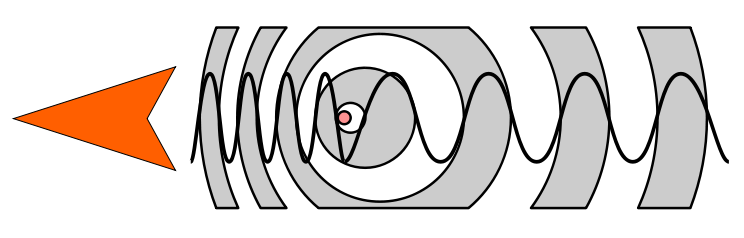
\includegraphics[width=3.5in]{doppler.png}
  \caption{The Doppler Effect illustrated.\cite{wiki}}
  \label{doppler}
\end{figure}

\par The Doppler effect has been adopted in a myriad of different ways over the last century and one very common and prominent application of the Doppler effect is to measure the speed of moving objects. Today this is commonly used in traffic cameras and the like and the way this works is by placing a transmitter and receiver along the road and having the transmitter send out a continuous high frequency signal, this signal will then bounce on oncoming vehicles and produce an echo which will be caught by the receiver. The echo will then have a different frequency as opposed to the original signal and by using the findings of Christian Doppler one can calculate the speed and direction of the object which produced the echo.
An illustration of this can be seen in figure 2.

\begin{figure}[!ht]
  \centering
  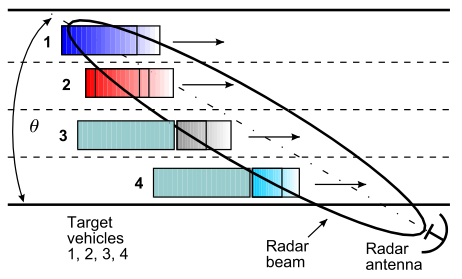
\includegraphics[width=3.5in]{radar.png}
  \caption{Doppler effect used for speed measuring in traffic.\cite{L6}}
  \label{radar}
\end{figure}

\section{Observations}
When looking at the signals from the movement of the fan it is of interest to study the Fourier transform of the signal echo, studying the signal on a digital oscilloscope will show something resembling figure 3 where we can clearly see the original signal (in this case 40kHz) and the frequency shifted signals produced by a object moving away from the sensor or towards the sensor.
\begin{figure}[!ht]
  \centering
  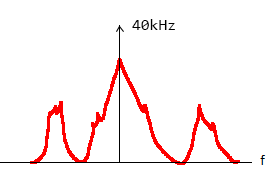
\includegraphics[width=3.5in]{transform.png}
  \caption{A very rough sketch of the transform of the signal received at the receiver.}
  \label{transform}
\end{figure}

\section{Method}
In order to utilize the Doppler effect to calculate the speed of an incoming or departing object we are first interested in finding the frequency shift, $f_{dk}$. The frequency shift can also be expressed as a function of the transmitted signal and the received echo giving us the following function:\\ 
\begin{equation}
f_{dk} = f_{rk} - f_0
\end{equation}
where $f_{rk}$ is the frequency of the received echo and $f_0$ the frequency of the transmitted signal. Now we also know that $f_{dk}$ can be expressed as a function of the velocity of the object $v_k$, the speed of sound $c$, the transmitted frequency $f_0$, and the angle of the sensor (see $\theta$ in figure 2). This gives us the following formula: 
\begin{equation}
f_{dk} = 2\frac{v_k}{c}f_0cos(\theta)
\end{equation}
Inserting equation (1) into equation (2) and solving for $v_k$ gives us:
\begin{equation}
v_k = \frac{c}{2cos(\theta)}(\frac{f_{rk}}{f_0}-1)
\end{equation}
In our implementation we know that the sensor will be at a angle $\theta = 45\degree$ so we can further simplify equation (3) into the following:
\begin{equation}
v_k = \frac{c}{\sqrt{2}}(\frac{f_{rk}}{f_0}-1)
\end{equation}
Now in order to find the direction of the object we are measuring we simply need to look at the ratio $\frac{f_{rk}}{f_0}$ since we know that the frequency of a object approaching the sensor will be higher and the frequency of a object departing from the sensor will be lower. Thus if the ratio $\frac{f_{rk}}{f_0} < 1$ we know that the object is departing from the sensor and if $\frac{f_{rk}}{f_0} > 1$ we know that the object is approaching the sensor.

\section{Implementation}
In order to implement the method above on the embedded system we make use of the Fourier transform of the incoming signal (the echo). We first find the index of the transmitted signal, at 40kHz. After this we use this index to partition the buffer into two partitions, one containing frequencies higher than 40kHz and one containing frequencies lower than 40kHz.
We then find the index of the spike in each partition which constitutes the lower and higher frequency of objects moving towards or departing from the sensor.
Finally we apply equation (4) on the lower and the higher frequency, convert that result to km/h and print it to PuTTy producing the following result:\\
\begin{figure}[!ht]
  \centering
  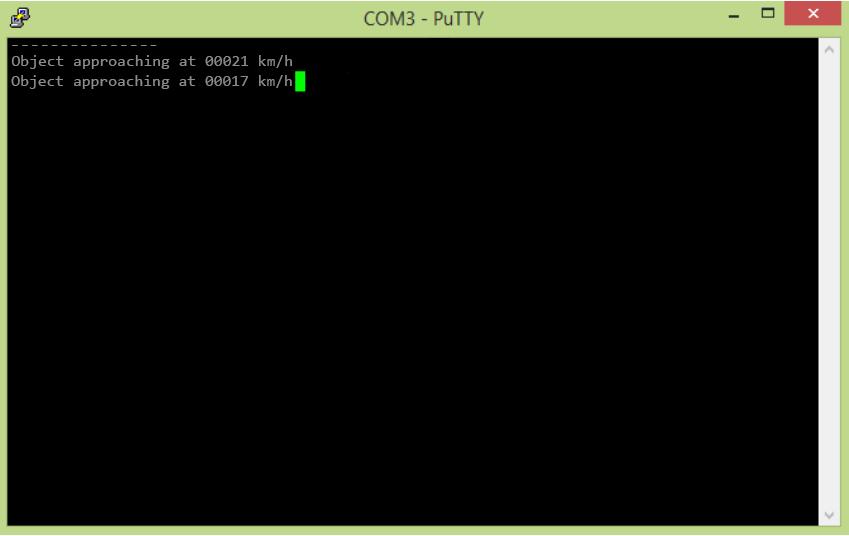
\includegraphics[width=3.5in]{putty.png}
  \caption{Example of PuTTy when running the embedded system.}
  \label{putty}
\end{figure}
\textit{The interested reader will find the entire c-code implementation in the appendix.}

\section{Performance evaluation}

The implementation that has been done is fairly robust in case of accuracy, resolution and detectability. This does not, however, mean that the system is a finished product. There are still some things that can be optimized even though the result are really good. 
The system determines the accuracy (or resolution) by dividing the sampling frequency in a specific amount of samples which in this case is 1024. If this sampling amount would be increased a better accuracy (or resolution) would be possible to acquire.

There are numerous factors that can affect the detectability of the system. Whereas our system can differentiate between a lorry and a small car is hard to say without empiric tests and observations. One thing is certain about the system that was implemented and that is that it didn't really have that much of an issue with distinguishing between the different fans. Something that was a concern when doing this was however how to position the fans correctly in order to get a good reading. How to improve this is easily done with hardware in form of a platform in which the measuring equipment and fans reside. If the solution were meant to be on the software side of the system then that is something that will have to be developed further.


\section{Results \& Discussion}
The implementation showed good results when showing measuring speed of both the departing fan and the approaching fan. It was easy to see whenever the speed of any fan decreased or increased. However as with all things the implementation was not perfect and even though the embedded managed to tell the speed fairly good there were also a lot of moments where it failed to produced reliable results, for instance showing the object as stand-still while it was in fact moving. This could be caused by the nature of signals since the echo from one fan could easily cause problems with the measurements of the other fans. We also notice that the exact placement of the sensor relative to the fans caused measuring problems where once you had good values you could get much worse values if you just shifted the fan slightly. \\
Another problem could be that the sound of the transmitted signal interferes with the receiver seeing as they are located close to each other.

\section{Conclusion}
In general the ultrasonic sensor serves as a good choice for measuring speed and even with the basic technology used to implement the system presented in this report we were still able to achieve somewhat reliable results. However as discussed in the report the implementation is not without fault and definitely not perfect. There are several problems that appeared during the implementation process but these problem can all be remedied by using more sophisticated equipment in an real-life situation as opposed to measuring fans in a lab to simulate moving objects. \\
All in all the project is deemed to be successful in producing a good, working, application of speed measurement.

\newpage
\section*{Appendix}

The c-code for the embedded system: \\
\begin{lstlisting}[frame=single]
	dsp16_trans_realcomplexfft(&DSP_COMP_BUFFER,&DSP_REAL_BUFFER,N_of_bits);
	dsp16_vect_complex_abs(&DSP_REAL_BUFFER,&DSP_COMP_BUFFER,DATA_SIZE);
	
	DSP_REAL_BUFFER[0]=0;
	DSP_REAL_BUFFER[1]=0;
	uint16_t speed = 330; //Speed of sound in air (m/s)
	
	volatile uint16_t max = dsp16_vect_max(&DSP_REAL_BUFFER,(DATA_SIZE/2));
	//find f0
	uint16_t f0_index;
	for(int i=0; i<=(DATA_SIZE/2); i++){
		if (max == (DSP_REAL_BUFFER[i])){
			f0_index = i;
			break;
		}
	}
	//find the indexes for the frequency shift
	volatile uint16_t lower_max = dsp16_vect_max(&DSP_REAL_BUFFER,(f0_index-2));

	uint16_t lower_index;
	for(int i=0; i<=(f0_index-2); i++){
		if (lower_max == (DSP_REAL_BUFFER[i])){
			lower_index = i;
			break;
		}
	}
	volatile uint16_t upper_max = dsp16_vect_max(&DSP_REAL_BUFFER[(f0_index+2)],((DATA_SIZE/2)-f0_index-2));

	uint16_t upper_index;
	for(int ind=(f0_index+2); ind<=(DATA_SIZE/2); ind++){
		if (upper_max == (DSP_REAL_BUFFER[ind])){
			upper_index = ind;
			break;
		}
	}
	
	//calculate delta frequency
	uint16_t delta_lower = dsp16_op_abs((lower_index-f0_index))*1000;
	uint16_t delta_upper = ((upper_index-f0_index)*1000);
	
	//calculate velocity
    uint16_t sqrt2 = 1.414;
	uint16_t out_velocity = (speed/sqrt2)*(delta_upper/f0_index);
	uint16_t inc_velocity = (speed/sqrt2)*(delta_lower/f0_index);
	inc_velocity = ((inc_velocity*18)/5)/1000;
	out_velocity = ((out_velocity*18)/5)/1000;
	//print results
	usart_write_line(USART, "\n\r---------------");
	usart_write_line(USART, "\n\rObject approaching at ");
	User_Usart_int2str(inc_velocity);
	usart_write_line(USART, " km/h");
	usart_write_line(USART, "\n\rObject departing at ");
	User_Usart_int2str(out_velocity);
	usart_write_line(USART, " km/h");	
\end{lstlisting}

\begin{thebibliography}{9}

\bibitem{wiki}
  Wikipedia,
  \emph{Doppler Effect}.
  http://en.wikipedia.org/wiki/Doppler\_effect

  \bibitem{L6}
  Ping Wu,
  \emph{Lab session 6: Correlation and Spectral Analysis}.
  Uppsala University,
  2015.

\end{thebibliography}

\end{document}